
\section{Introducción}

Esta sección se enfocará a la parte de transmisión de información y tipo de operaciones lógicas matemáticas que ocurren para que un cerebro pueda realizar cómputos. Específicamente se detallará la mecánica de los disparos de las neuronas, siendo estos una de las características más relevantes a la hora de modelar las redes neuronales artificiales. Si en algún momento de su vida han visto temas relacionados con: compuertas digitales, arquitectura de computadoras o diseño electrónico digital, les será más fácil abstraer el concepto, pues vamos a ver los procesos de paso de información a través de compuertas pero en un sistema biológico (de la naturaleza). 

Notemos primeramente un impulso nervioso, recordemos que esté es una onda que avanza desde el cono axónico de la neurona hasta la neurona postsináptica. Esta onda electroquímica ocurre dada la diferencia de potencial entre la parte interna y externa de neurona, está diferencia se da a consecuencia de las distintas concentraciones de iones en ambos lados de la membrana plasmática. Los estados en la membrana plasmática (del axón) se pueden diferenciar en, potenciales neuronales:

\begin{itemize}
\item \textbf{Potencial de reposo:} Es la diferencia de cargas en la membrana y está polarizada a -70 mV. Es positiva por fuera (Na+) y negativa por dentro por Cl- y proteínas- y no transmite señal. 
\item \textbf{Potencial de acción o membrana:} Un estímulo umbral de 55 mV, despolariza la membrana y abre los canales del Na+ y K+ y avanza la señal nerviosa, es un cambio muy rápido en la polaridad de la membrana de negativo a positivo y vuelta a negativo.
\end{itemize}

%(Insertar esquema) 
\begin{figure}[h]
 \centering
 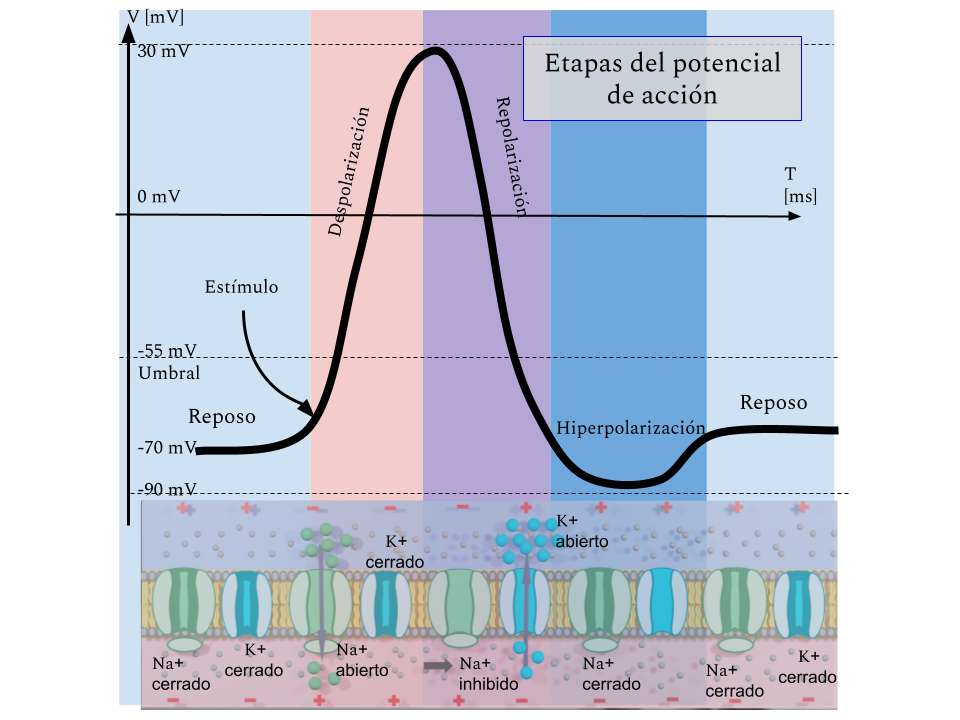
\includegraphics[scale=0.5]{../Figuras/Grafica.png}
 \caption{Representación gráfica de la respuesta de los canales iónicos de sodio (Na+ en verde) y potasio (K+ en azul) ante un estímulo de voltaje, dando como resultado un potencial de acción que viajará a lo largo de todo el axón.}
 \label{fig:graficaP}
\end{figure}

Retomando la sinapsis eléctrica, donde participan los canales iónicos y las entradas de las neuronas (dendritas) están siendo alteradas poco a poco, hasta que ocurre la suficiente carga (diferencia de potencial) en sus dendritas y en el cuerpo de la neurona, para que desde el cono axónico sé dé un disparo o potencial de acción (spike), transmitiendo la información gracias a la apertura y cierre de ciertos canales de iones cargados. Este cambio brusco de la diferencia de potencial, se nota en forma de un pulso eléctrico (ver \ref{fig:graficaP}), para saber más a detalle qué está ocurriendo en esta rápida elevación en la diferencia de potencial, se contará de dónde salió este modelo y por qué toma la forma que tiene. 

Los primeros científicos que estudiaron el potencial de acción y dieron un modelo (de la unión sináptica eléctrica) fueron Alan Lloyd Hodgkin y Andrew Fielding Huxley alrededor de 1952, obteniendo un modelo matemático \footnote{El texto original de este experimento se puede encontrar en la siguiente url: \url{ https://physoc.onlinelibrary.wiley.com/doi/pdf/10.1113/jphysiol.1952.sp004764}}, que intenta explicar qué es lo que estaba pasando en las neuronas. Ellos trabajaron con un calamar gigante (que puede medir hasta 4 metros de largo) que dado su gran tamaño, tiene un axón también bastante gigantesco, que recorre casi la mitad del cuerpo del calamar y su grosor es de medio milímetro, considerando el tamaño estándar de un axón de una neurona (1-20 µm). El axón del calamar gigante es tan grande que les permitió introducir dispositivos para medir el voltaje, es decir, la diferencia de potencial entre, el interior de la neurona y la parte de afuera (el ambiente externo de la neurona). Con estas mediciones experimentales que lograron obtener, se pudo determinar qué pasaba con las cargas eléctricas tanto en el interior como en el exterior y así estudiar cómo se lograba la transferencia de electricidad cuando disparaba este pulso. 
 Se dan cuenta de que podían modelar este comportamiento como un circuito eléctrico donde están corriendo estas corrientes, si bien aún no sabían todavía cuál era exactamente el mecanismo biológico por detrás, si observaron que había dos elementos protagónicos que serían el sodio y el potasio.
 Notaron que estos existen en diferentes concentraciones, en la parte de afuera y en la parte de adentro de las neuronas. Con esto nosotros podemos aprender también el por qué es importante consumir algo de sal y nunca estar bajos de potasio, pues estos dos elementos son indispensables para que las neuronas puedan transmitir sus señales. 

\section{Membrana y canal}

Hodgkin y Huxley se dedicaron a estudiar qué pasaba con las concentraciones de estos iones (sodio y potasio) en la parte de afuera o en la parte de adentro cuando empezaban a fluir las corrientes. El sistema parecía una especie de circuito eléctrico, se lo imaginaron como una especie de membrana porosa (lo cual es bastante cercano a lo que después se descubrió con la microscopía) y la forma en que lo vieron fue como un circuito eléctrico donde \textit{la membrana está funcionando como un capacitor} que almacena ligeramente las cargas cuando están tratando de pasar de un lado hacia el otro y además con la cualidad que tenía de veces dejar pasar más iones y a veces no (semipermeable), modelan esto como una especie de \textit{resistencias variables}. Bajo ciertas condiciones de voltaje de la diferencia de potencial entre la parte de afuera y la parte de adentro, estos canales permiten pasar más de estos iones (ya sean sodio, potasio o calcio) o, por el contrario, impiden su paso (ver \ref{fig:ModelHh}).


\begin{figure}[h]
 \centering
 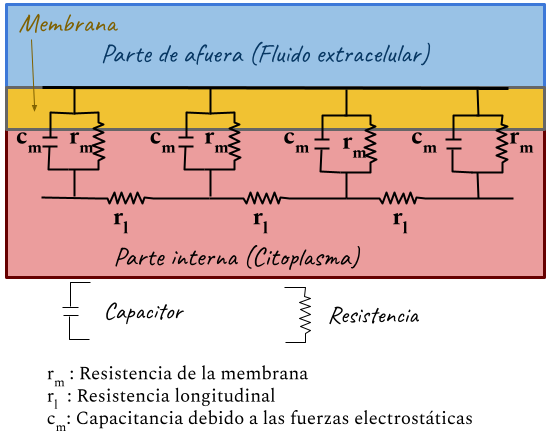
\includegraphics[scale=0.5]{../Figuras/ModeloHH.2}
 \caption{Un primer modelo de la membrana axónica modelada como circuito eléctrico. La parte amarilla es la membrana.}
 \label{fig:ModelHh}
\end{figure}


Ahora se necesitan más detalles de la representación de los canales y toman en cuenta que el comportamiento de estas resistencias viene acompañado con un voltaje de reposo, en estos voltajes particulares cada tipo de ion (de la resistencia modelada) se estabiliza y ya no va a cambiar esta resistencia (ver \ref{fig:circuito}). 


\begin{figure}[h]
 \centering
 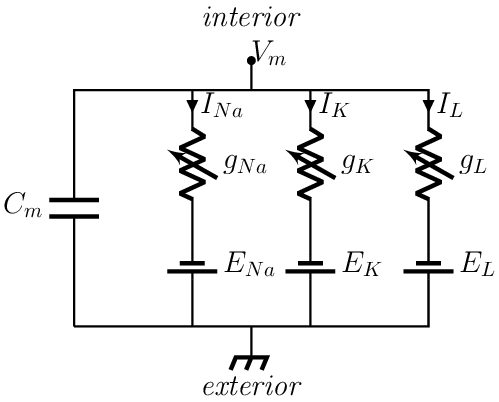
\includegraphics[scale=0.5]{../Figuras/circuito.png}
 \caption{Modelo de la membrana axónica modelada como circuito eléctrico, con los distintos canales presentes y su voltaje de reposo.}
 \label{fig:circuito}
\end{figure}

Lo que observan es que el \textbf{ion de sodio (Na+)} y su resistencia va a variar dependiendo del voltaje, a esto se le llama un \textbf{canal transitorio} porque en ciertos voltajes si puede pasar; si es muy bajo, no puede pasar y si rebasa un cierto umbral entonces se vuelve a tapar y ya no puede pasar. 
Lo que sucede con el \textbf{ion de potasio (K+)} es que, puede salir si el voltaje está más allá de un cierto valor, si no, no pasan y va variando un poquito que tanto puede pasar, a esto se le llama \textbf{canal persistente}. Por estas características de que el potasio es un intervalo dentro de la recta y el sodio es a partir de cierto valor, por tanto, se les modelan de maneras ligeramente diferentes. Más adelante se descubrió porque tenían este comportamiento, básicamente el canal de potasio es una puerta hecha de cuatro subpuertas por donde los elementos pasan o no pasan, el canal de sodio es como una compuerta que está hecha de tres subpuertas que se pueden abrir y tiene aparte un tapón extra, que hace que aunque estas tres están abiertas bloquee toda la compuerta.
Las neuronas están trabajando con muchos más iones aparte de estos dos, uno que destaca bastante es el caso del cloro (Cl-) que tiene carga negativa. Se tienen canales para intercambio aleatorio de otros iones, \textbf{L} un canal aleatorio (leaky).

Entonces con lo que ellos midieron experimentalmente, notaron cómo se estaban comportando estas resistencias dependiendo del voltaje o la diferencia de potencial que había entre ambos lados de la membrana. A partir de estas pudieron describir matemáticamente y simular los disparos que se conocen como potenciales de acción. Vamos a ver cuáles fueron estos conceptos de electricidad que se están utilizando para el modelo tenemos este concepto de potenciales eléctricos.

\begin{itemize}
\item Potenciales eléctricos \emph{E ó  V}; resultan de la separación de cargas opuestas. Se mide en \emph{mV}.
    \begin{itemize}
     \item \emph{E\textsubscript{(Na,K,L)}} voltaje en reposo para los iones de Na, K y L, o también conocido como  potencial de inversión iónico, es el potencial de membrana en el que no hay flujo neto (total) de ese ion en particular de un lado de la membrana al otro. 
     \item \emph{V\textsubscript{m}}, el potencial eléctrico de la membrana. 
     \end{itemize}

\item Corriente \emph{I}; Movimiento de cargas. Se mide en \emph{µA}.
    \begin{itemize}
     \item \emph{I\textsubscript{(Na,K,L)}} corriente entrante a los canales de Na, K o L.
     \end{itemize}

\item Resistencia \emph{R}; Medida de la oposición al movimiento de las partículas cargadas.
\item Capacitancia o capacidad eléctrica \emph{C} . Cantidad de energía eléctrica almacenada en un capacitor para una diferencia de potencial eléctrico dada.
    \begin{itemize}
     \item \emph{C\textsubscript{m}} la capacitancia de la membrana. 
     \end{itemize}

\item Conductancia \emph{g}; Inverso de la resistencia \( \dfrac{1}{R} \) , es decir, facilidad de transmisión de las partículas cargadas.
    \begin{itemize}
     \item \emph{g\textsubscript{(Na,K,L}}  la conductancia del canal de sodio, potasio, cloro y la L también refiriendose a otros canales de iones. 
     \end{itemize}

\end{itemize}

Lo que está pasando en los \textbf{potenciales eléctricos} es que hay mucho sodio en la parte externa de la membrana por ej. tres iones de sodio que son cargas positivas por dos iones de potasio que hay en la parte interna, entonces hay muchas más cargas positivas en la parte de afuera que las que hay en la parte de adentro y eso es lo que provoca la diferencia de cargas que es lo que estamos viendo como un potencial eléctrico.


La capacidad eléctrica o \textbf{capacitancia} es la que estamos utilizando para modelar la membrana conformada por lípidos, que es una capa de grasa y esa es la cantidad de energía eléctrica almacenada en un capacitor para una diferencia de potencial eléctrico dada. Éste comportamiento bastante interesante porque las cargas quedan almacenadas un momento, pero se van liberando poco a poco y se va descargando ese capacitor. 


Durante el experimento con el axón, se le dieron cargas eléctricas directamente al axón y gracias a eso lograban ir midiendo que era lo que estaba pasando con las concentraciones de cargas afuera y adentro en el caso de las neuronas reales, esto en un ambiente no alterado ocurre cuando entran en juego los neurotransmisores y provocan que haya cambios, en estas corrientes. Entonces Hodgkin y Huxley jugaron el rol que tendrían que jugar usualmente los \emph{neurotransmisores} para abrir otras compuertas. Nosotros en la manera en la que lo vamos a simular es precisamente con estas corrientes que son las que se están poniendo en el experimento y vamos a ver cómo reacciona el axón. 


\section{Potenciales de Nerst o de reposo}

Los Potenciales de Nerst o de reposo son los potenciales a los cuales el flujo neto de iones a través de los canales abiertos es cero.
Aquí vemos precisamente porque estamos utilizando la \emph{E} generalmente la vamos a utilizar para referirnos a la diferencia de potencial entre la parte de afuera de la célula y la parte de adentro, las vamos a utilizar para representar a aquellos voltajes donde cada una de las compuertas encontrarían su equilibrio. Estos voltajes son distintos para cada una de las compuertas, esto va a provocar precisamente la dinámica de la de la neurona, por ejemplo: 

\begin{itemize}
\item E \textsubscript{Na}  \emph{50mV}
\item E \textsubscript{Ca}  \emph{150mV}
\item E \textsubscript{K}   \emph{− 80mV}
\item E \textsubscript{Cl}  \emph{− 60mV}
\end{itemize}

Aquí vemos que el sodio estaría su equilibrio en un valor positivo, 
el calcio que es el que va a jugar un rol de que se activen los neurotransmisores y se transmita el disparo, observamos que el voltaje tendría que ser bastante positivo. El potasio que es el que usualmente está trabajando intercambiándose casi todo el tiempo en la neurona, veremos que el punto de equilibrio usual de la neurona anda por los $-76 mV$ y el del cloro. Cada uno de estos canales pues está tratando de jalar la dinámica hacia su potencial de equilibrio y no hay precisamente un acuerdo entre ellos y eso es precisamente lo que hace que las neuronas cobren "vida".


\section{Modelo de la membrana como bicapa de lípidos}

\hypertarget{LaEq}{La membrana} de una neurona es modelada como un elemento de un circuito con capacitancia \emph{C\textsubscript{m}} y potencial \emph{V}, las corrientes que fluye a través de la bicapa lipídica están regidos por las siguientes ecuaciones:


\begin{equation}
  I_{m} = C_{m} \dfrac{dV_{m}}{dt}
  \label{eq:corrientesEnLaMembrana}
\end{equation}

Esta sería la ecuación principal (\ref{eq:corrientesEnLaMembrana}) donde \(\dfrac{dVm}{dt}\) está representando el cambio voltaje en la membrana respecto al tiempo.

\begin{equation}
  C_{m} \dfrac{dV_{m}}{dt} =  - g_{Na} m^3 h(V - E_{Na} ) - g_{K} n 4 (V - E_{K} ) - g_{L} (V - E_{L} ) + I_ext
  \label{eq:corrientesEnLaMembrana2}
\end{equation}

Cada una de las partes del lado izquierdo de la ecuación \ref{eq:corrientesEnLaMembrana2} corresponde a las compuertas de los canales y la corriente de un estímulo externo que pueda influir a la membrana (este estímulo siempre será desde al exterior hacia el interior).

Retomando lo escrito anteriormente el canal de sodio es una compuerta compuesta de \textbf{tres} subpuertas y una subpuerta que actua como tapón y el canal de potasio es una compuerta compuesta de \textbf{cuatro} subpuertas iguales, \hypertarget{secc} {con esto podemos notar claramente que las conductancias sean representadas como}:

\begin{itemize}
 \item \(\dfrac{1}{R_{Na}} = g_{Na} * m ^3 * h \) donde \(g_{Na}\) es una constante que representa el valor de la conductancia máxima, \textbf{m} es la proporción de los canales de sodio abiertos (representa la concentración de sodio) y nos indica la activación (subpuertas abiertas) del canal, \textbf{h} es el “tapón” de la compuerta que puede impedir el paso de iones independientemente de las otras tres subpuertas, es decir la inactivación (compuerta bloqueada).
Los movimientos combinados de \textbf{m} y \textbf{h} son los que controlan la compuerta de sodio.
 \item \(\dfrac{1}{R_{K}} = g_{K} * n^4\) donde \(g_{K}\) es una constante que representa el valor de la conductancia máxima, \textbf{n} es la proporción de los canales de potasio abiertos (representa la concentración de potasio) y nos indica la activación del canal de potasio.
 \item \(g_{L}\) es una constante, de los canales por fuga, que representa la concentración de los demás iones que pasan por la membrana.
\end{itemize}

Ahora \emph{m}, \emph{n} y \emph{h}, son variables de activación que describen la probabilidad de que los canales iónicos estén abiertos, se puede describir mediante las siguientes ecuaciones diferenciales ordinarias:

\begin{equation}
  \dfrac{1}{\gamma(T)}\dfrac{dn}{dt} =  \alpha_{n^\infty} (V)(1 - n) - \beta_{n} (V) n = \dfrac{n(V)-n(t)}{\tau_{n}(V)}
  \label{eq:corrientesEnLaMembrana3}
\end{equation}

\begin{equation}
  \dfrac{1}{\gamma(T)}\dfrac{dm}{dt} =  \alpha_{m} (V)(1 - m) - \beta_{m} (V) m = \dfrac{m^\infty(V)-m(t)}{\tau_{m}(V)}
  \label{eq:corrientesEnLaMembrana4}
\end{equation}

\begin{equation}
  \dfrac{1}{\gamma(T)}\dfrac{dh}{dt} =  \alpha_{h} (V)(1 - h) - \beta_{h} (V) h = \dfrac{h^\infty(V)-h(t)}{\tau_{h}(V)}
  \label{eq:corrientesEnLaMembrana5}
\end{equation}

Donde la ecuación \ref{eq:corrientesEnLaMembrana3} representa al canal de potasio y las ecuaciones \ref{eq:corrientesEnLaMembrana4} y \ref{eq:corrientesEnLaMembrana5} representando al canal de sodio tomando en cuenta que tiene dos tipos de subpuertas.

Las expresiones de \(\alpha\) y \(\beta\) están dadas por las siguientes ecuaciones:

\begin{align*}
\alpha_{n}&=\dfrac{0.01(10-V)}{exp(\dfrac{10-V}{10})-1}           &  \beta_{n}&=0.125exp-\dfrac{V}{80}\\
\alpha_{m}&=\dfrac{0.01(25-V)}{exp(\dfrac{25-V}{10})-1}                    &  \beta_{m}&=4exp-\dfrac{V}{18}\\
\alpha_{h}&=\dfrac{0.07}{exp-(\dfrac{V}{20})}              &  \beta_{h}&=\dfrac{1}{1+exp\dfrac{30-V}{10}}
\end{align*}

Los factores \(\alpha\) y \(\beta\) se denominan como constantes de velocidad de transición. \(\alpha\) es el número de veces por segundo que se abre una puerta que está en estado cerrado, mientras que \(\beta\) es el número de veces por segundo que se cierra una puerta que está en estado abierto. Si la membrana tiene un la carga negativa, \(\alpha\) debe aumentar y la \(\beta\) debe disminuir, cuando la membrana esté despolarizada.

Hasta ahora sabemos que en la bicapa de lípidos, una pequeña carga está pasando entre sus capas de grasa. También sabemos que la carga es almacenada por un breve periodo de tiempo, dando como resultado que la bicapa se comporte como un \textbf{capacitor}. Esta membrana también está con cierta resistencia al paso de corriente. Con esto tenemos el siguiente diagrama \footnote{Otra explicación más profunda de las ecuaciones dadas partir del diagrama \ref{fig:circuitoP}la podemos encontrar en \url{https://neurowiki.case.edu/wiki/Action_Potential_IV:_Hodgkin-Huxley_Equations_and_Other_Conductances}} \ref{fig:circuitoP}

\begin{figure}[h]
 \centering
 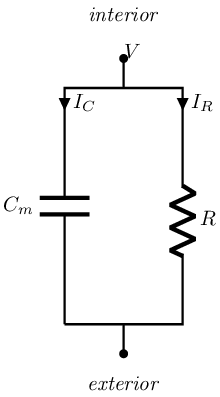
\includegraphics[scale=0.5]{../Figuras/bicapaLipidos.png}
 \caption{Modelo de la bicapa de lipidos donde, V son los cambios de voltaje en la membrana que es el potencial eléctrico, \(I_{C}\) es la corriente del capacitor, \(I_{R}\) es la corriente de la resistencia, \(C_{m}\) es la capacitancia de la membrana, R es la resistencia.}
 \label{fig:circuitoP}
\end{figure}

Tenemos dadas las siguientes ecuaciones:
\begin{equation}
    I_{C} + I_{R} - I_{ext} = 0
  \label{eq:bicapa1}
\end{equation}

\begin{equation}
    C\dfrac{dV}{dt} + \dfrac{V}{R} - I_{ext} = 0 \\
  \label{eq:bicapa2}
\end{equation}

\begin{equation*}
    C\dfrac{dV}{dt} = -\dfrac{V}{R} + I_{ext} 
\end{equation*}

Ahora por la ley de corriente de Kirchhoff \footnote{La ley de la corriente de Kirchhoff dice que la suma de todas las corrientes que fluyen hacia un nodo es igual a la suma de las corrientes que salen del nodo} tenemos que la suma de las corrientes del capacitor y la resistencia debe ser cero
por la conservación de corriente y si consideramos un factor adicional de una corriente externa aplicada o administrada a la neurona, tenemos la ecuación \ref{eq:bicapa1}.

Después tenemos la relación entre la diferencia de potenciales, que almacena energía y la carga eléctrica que guarda, donde: \emph{C} es la capacidad, medida en faradios, \emph{Q} la carga eléctrica almacenada, medida en culombios, \emph{V} la diferencia de potencial medida en voltios. Entonces \(C = Q/V\), despejando a \emph{Q} tenemos \emph{Q = CV} y derivando de ambos lados respecto al tiempo y considerando que \emph{C} es una constante al ser una propiedad de la membrana \(\dfrac{dQ}{dt} = C\dfrac{dV}{dt}\). Como la definición de corriente es el cambio de carga en el tiempo tenemos que \(I_{C} = C\dfrac{dV}{dt}\). Notemos finalmente la corriente de la resistencia \(I_{R}\), recordando la ley de Ohm \footnote{La ley de Ohm establece que la diferencia de potencial V que aplicamos entre los extremos de un conductor determinado es directamente proporcional a la intensidad de la corriente I que circula por el conductor, es decir \(V = R * I\). Notemos también que \(V = V_{m} - V_{rest}\) } la podemos rescribir como \(\dfrac{V-V_{rest}}{R}\). Sustituyendo de lo anterior en la ecuación \ref{eq:bicapa1} se obtiene la siguiente ecuación:

\begin{equation}
 C\dfrac{dV}{dt} + \dfrac{V-V_{rest}}{R} - I_{ext} = 0
 \label{eq:bicapa3}
\end{equation}

\begin{equation*}
 C\dfrac{dV}{dt} = -\dfrac{V-V_{rest}}{R} + I_{ext} 
\end{equation*}

Ahora multiplicando todo por R:
\begin{equation}
 RC\dfrac{dV}{dt} = -V + (V_{rest} + RI_{ext}) 
 \label{eq:bicapa4}
\end{equation}

Denotando RC como la constante de tiempo \(\tau\) y tomando en cuenta que en cuanto se aplica la corriente va a empezar a cambiar el voltaje poco a poco hasta establecerse en un voltaje de equilibrio (ahí se va a quedar quieta). Entonces cuando el voltaje ya no está cambiando con el tiempo quiere decir que su derivada con respecto al tiempo es cero. Observemos que \(dV/dt = 0\) significaría que V es igual a infinito y que el voltaje en el estado estacionario cuando, \(dV/dt = 0\) depende del potencial de reposo y del producto entre la resistencia con la corriente externa suministrada, entonces tenemos que:

\begin{equation}
 V_{\infty} = V_{rest} + RI_{ext}
 \label{eq:bicapa5}
\end{equation}

Sustituyendo con \ref{eq:bicapa5} y la constante, en \ref{eq:bicapa4} tenemos que:
\begin{equation}
 \tau\dfrac{dV}{dt} = -V + V_{\infty}
 \label{eq:bicapa6}
\end{equation}

\subsection{Las conductancias iónicas}
Nuestro objetivo aquí es encontrar ecuaciones que describan las conductancias con precisión razonable y lo suficientemente simples para el cálculo teórico de \emph{el potencial de acción} y \emph{el período refractario}. 

Si tomamos las ecuaciones diferenciales anteriores notamos que las soluciones tienen este tipo de forma \ref{fig:graficaX}:

\begin{figure}[h]
 \centering
 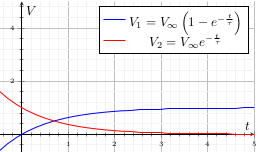
\includegraphics[scale=0.8]{../Figuras/solPulso1.png}
 \caption{Soluciones para el pulso.}
 \label{fig:graficaX}
\end{figure}


Donde si estamos aplicando una corriente externa lo que sucede es lo que estamos viendo en azul, un exponencial que va creciendo y que tiende hacia un cierto valor límite que sería de infinito. Si dejamos de aplicar la corriente externa entonces ahora tendremos un exponencial, pero que tiende hacia el cero y se va a estabilizar en cero, lo que vemos en rojo. 

\begin{figure}[h]
 \centering
 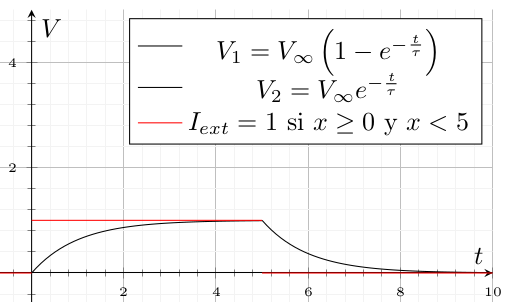
\includegraphics[scale=0.5]{../Figuras/solPulso2.png}
 \caption{Soluciones para el pulso escalón.}
 \label{fig:graficaX1}
\end{figure}

Simulando lo que hicieron Hodgkin y Huxley que fue al axón de repente darle un toque, siendo en el origen de la gráfica (que visualizamos en la figura \ref{fig:graficaX1}) la parte en la que le están dando el toque al axón, momentos antes estaba quieta la neurona de repente le aplican una cierta cantidad de electricidad y va a empezar a cambiar el comportamiento de los canales la porosidad de la membrana, vamos a ver que empieza a incrementarse la diferencia de potencial hasta que llegan a un nuevo equilibrio (alrededor de t = 3) y si siguieran dándole el toque en esa cantidad se quedaría ahí la neurona, ya no veríamos más cambios lo que va a suceder entonces es que, retiramos las pinzas (se le deja de dar el toque) y los canales otra vez van a empezar a regresar a la normalidad y vamos a ver un descenso en adelante.

Entonces hasta aquí ya tenemos la idea de cómo va a reaccionar la neurona ante cierto estímulo; sin embargo, esto que acabamos de ver en las gráficas sería como si tuviéramos un solo tipo de canal, ahora qué pasa si consideramos que tenemos diferentes tipos de canales pasando iones, en condiciones distintas. 
Aquí es donde va a importarnos el hecho de que existen diferentes tipos de canales con voltajes de equilibrio diferente. 
Retomando a los potenciales de Nerst \(E_{Na},E_{K},E_{L}\) notemos que están dados por:


\begin{equation}
    E = \dfrac{k_{B}T}{zq}\ln\dfrac{[adentro]}{[afuera]}
 \label{eq:diferenciaP}
\end{equation}

Estos potenciales están relacionados con las características termodinámicas, en la ecuación anterior \ref{eq:diferenciaP} \(k_{B}\) la constante de Boltzman, \(q\) es la carga del ion, y \(z\) es el número de iones. El logaritmo natural representando el promedio de cuántos elementos tenemos en la parte de adentro con respecto a cuántos elementos tenemos en la parte de afuera.

Considerando los diferentes puntos de equilibrio en los cuales se puede encontrar la diferencia de potencial en la membrana, vamos a distinguir entre tres estados de esta (también se puede ver en \ref{fig:graficaP}):

\begin{enumerate}
 \item \textbf{Polarizada} en su estado de reposo con \(V < 0 ( V \approx -70 mV )\).
 \begin{itemize}
  \item Su estado de reposo,cuando la neurona no está haciendo nada simplemente están corriendo los sodios y entran los potasios.
 \end{itemize}
 \item \textbf{Despolarizada} cuando \(V \geq 0\).
 \begin{itemize}
  \item Cuando en sus dendritas y en el cuerpo de la neurona se acumula una carga muy grande (un voltaje electrico, disparo), se abre la compuerta de sodio y van a empezar a entrar el sodio, esta diferencia de potencial que existía entre lo fuera y lo adentro se va a reducir de hecho se puede llegar a reducir bastante dependiendo de la carga que se le aplique.
  \item Iones positivos entran a la membrana.
  \item Valores positivos en la diferencia de potencial.    
 \end{itemize}
 \item \textbf{Hiperpolarizada} cuando la diferencia de potencial incrementa su magnitud \(V << 0\).
 \begin{itemize}
 \item En cuanto se despolarice van a empiezar interacciones entre los diferentes tipos de canales que lo que van a intentar hacer es regresar a la neurona en su estado normal.
 \item Los canales de potasio abren sus compuertas, provocando que salga el potasio que está dentro del axón (en el citoplasma). 
 \item Iones positivos salen de la membrana.
 \item Si antes estaba quieta a los - 70mV, ahora va a quedar todavía más abajo alrededor de - 90mV. Esto va a permitir un fenómeno que se le conoce como \emph{el periodo de refracción} y ese periodo sirve para que simplemente se lance un disparo y que el comportamiento eléctrico no se rebote otra vez en dirección contraria en la neurona, va a quedar muy quieta la neurona durante un rato y después regresará otra vez a su estado de equilibrio. 
 \end{itemize}

\end{enumerate}
 
\section{Modelo de las compuertas iónicas controladas por voltaje}

Retomando el modelo del circuito eléctrico modelando la membrana, junto con los canales y los iones, volvamos a verlo ahora en la \ref{fig:circuito1}

\begin{figure}[H]
 \centering
 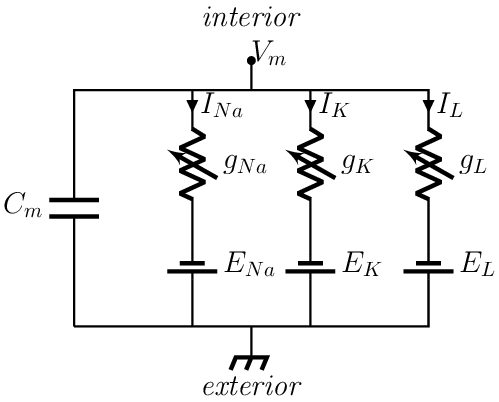
\includegraphics[scale=0.5]{../Figuras/circuito.png}
 \caption{Modelo de la membrana axónica modelada como circuito eléctrico, con los distintos canales presentes y su voltaje de reposo.}
 \label{fig:circuito1}
\end{figure}

Recordemos brevemente las definiciones de los dos tipos de canales protagonistas en el modelo:

\begin{definition}
 \emph{Canal persistente} Tiene un solo tipo de compuerta y dos estados posibles:
 \begin{enumerate}
  \item \textbf{Activado}
  \item \textbf{Desactivado}
 \end{enumerate}

\end{definition}

\begin{definition}
 \emph{Canal transitorio} Tiene compuertas de activación e inactivación, y tres estados:
 \begin{enumerate}
  \item \textbf{Activado} Ambas compuertas abiertas.
  \item \textbf{Desactivado} Compuerta de activación cerrada, inactivación abierta.
  \item \textbf{Inactivada} Compuerta de inactivación cerrada.
 \end{enumerate}

\end{definition}


Y retomando \hyperlink{LaEq}{la primera ecuación diferencial} donde tenemos, por un lado, la corriente que está pasando a través del capacitor, por otro lado, vamos a tener las corrientes que están circulando a través de los diferentes canales, 

\begin{equation}
  C_{m} \dfrac{dV_{m}}{dt} = - g_{Na} m^3 h(V_{m} - E_{Na}) - g_{K} n 4 (V_{m} - E_{K}) - g_{L} (V_{m} - E_{L}) + I_{ext}
  \tag{\ref{eq:corrientesEnLaMembrana2}}
\end{equation}

Las capacitancias y variables del lado izquierdo están explicadas en la sección \hyperlink{secc}{\emph{Modelo de la membrana como bicapa de lípidos}}, aqui vamos a retomar las ecuaciones \ref{eq:corrientesEnLaMembrana3},\ref{eq:corrientesEnLaMembrana4},\ref{eq:corrientesEnLaMembrana5} de esa misma sección, (recordemos que estás ecuaciones describen la probabilidad de que los canales iónicos estén abiertos) que son las siguientes:

\begin{equation}
  \dfrac{1}{\gamma(T)}\dfrac{dn}{dt} =  \alpha_{n^\infty} (V)(1 - n) - \beta_{n} (V) n = \dfrac{n(V)-n(t)}{\tau_{n}(V)}
  %\label{eq:probabilidades1}
  \tag{\ref{corrientesEnLaMembrana3}}
\end{equation}

\begin{equation}
  \dfrac{1}{\gamma(T)}\dfrac{dm}{dt} =  \alpha_{m} (V)(1 - m) - \beta_{m} (V) m = \dfrac{m^\infty(V)-m(t)}{\tau_{m}(V)}
  %\label{eq:probabilidades2}
  \tag{\ref{corrientesEnLaMembrana4}}
\end{equation}

\begin{equation}
  \dfrac{1}{\gamma(T)}\dfrac{dh}{dt} =  \alpha_{h} (V)(1 - h) - \beta_{h} (V) h = \dfrac{h^\infty(V)-h(t)}{\tau_{h}(V)}
  \tag{\ref{corrientesEnLaMembran53}}
\end{equation}

Ahora notemos los elementos en estas ecuaciones anteriores con \(ion\) pudiendo denotar las compuertas del potasio \(n\) o del sodio, ya sea \(m\) o \(h\):
\begin{itemize}
 \item \(\dfrac{1}{\gamma(T)}\) Este es el coeficiente de escala temporal, dependiente de la temperatura los por eso está apareciendo aquí una \(t\). Para las simulaciones que nosotros vamos a hacer vamos a pensar que estamos en una temperatura fija. 
 \item \(\alpha_{ion}(V)\) probabilidad de que una compuerta transite de cerrada a abierta.
 \item \(\beta_{ion}(V)\) probabilidad de que una compuerta transite de abierta a cerrada.
 \item \(ion^\infty(V)\) probabilidad de compuerta abierta en el equilibrio cuando \(t \rightarrow \infty\).
 \item \((ion)\) Probabilidad de que cada compuerta (n, m, h) esté abierta.
 \item \((1-ion)\) Probabilidad de que cada compuerta (n, m, h) esté cerrada.
 
 \item \(\tau_{ion}(V)\) Tiempo que toma llegar al equilibrio.
\end{itemize}


Lo que vamos a ver es que forma de escribir la ecuación depende precisamente del número de compuertas que tenían para poder abrirse y cerrarse. Reescribir la ecuación de esta manera lo que nos permite es medirlo en términos de estas probabilidades de que se abran y cierren las compuertas que serían 

Esta probabilidad se empieza a alterar conforme cambiamos el voltaje, pero no va a llegar a su valor de equilibrio sino hasta después de pasado un cierto periodo.


\section{Dinámica del voltaje durante un disparo} 

Ahora qué pasa cuando tomamos en cuenta que todas las compuertas están reaccionando al mismo tiempo.
Notemos primeramente como está reaccionando la membrana ante un impulso electrico o voltaje, en la siguiente imagen \ref{fig:voltaje1}.

\begin{figure}[h]
 \centering
 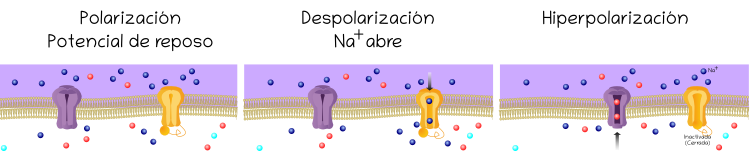
\includegraphics[scale=0.5]{../Figuras/polarizacion1.png}
 \caption{En la primera parte los canales están en un estado de reposo y la membrana está polarizada. En la segunda parte los canales han sido afectados por un impulso recibido desde el cono axónico, las compuertas de sodio se abren permitiendo el paso de iones de sodio al interior de la membrana y dejando a la membrana despolarizada. Momentos después la membrana llega a un estado de hiperpolarización donde intentará regresar al estado de equilibrio que tenía previamente, para esto la subpuerta de inactivación de sodio cerrará hasta no permitir el paso de sodio y el canal de potasio abrirá sus compuertas para dar salida a los potasios (iones positivos) que fluyan hacia el exterior de la membrana, así dejando el voltaje de la membrana incluso más negativo de lo que tenía durante su estado polarizado. }
 \label{fig:voltaje1}
\end{figure}

Ahora lo que vemos en la imagen \ref{fig:voltaje1} se grafica de manera un poco más apegada a lo que pasa en los experimentos de la siguiente forma en la imagen \ref{fig:voltaje2}.

\begin{figure}[h]
 \centering
 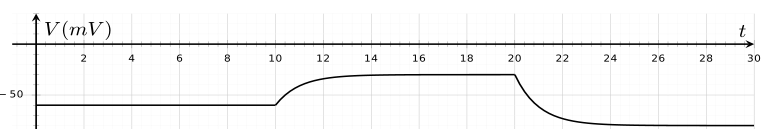
\includegraphics[scale=0.5]{../Figuras/polarizacion2.png}
 \caption{Gráfica del cambio de voltaje en la membrana dado un impulso atrevés del tiempo. Cuando se rebasa el voltaje umbral, los canales de Na + y K + interactúan para producir una rápida despolarización de la membrana provocando una elevación del voltaje, para luego hiperpolarizarla. Durante el momento de despolarización la membrana puede llegar a valores positivos en este caso en particular el estímulo no es tan grande y se queda en valores negativos.}
 \label{fig:voltaje2}
\end{figure}


Ahora lo anterior está en términos de lo deseado, veamos entonces que paso en las mediciones de Hodgkin y Huxley con el axón en las siguientes gráficas \ref{fig:voltajeAB}, donde nos está mostrando como las subpuertas n y los factores \(\tau\), \(\alpha\) y \(\beta\) del canal de potasio se comportaron antes, durante y después del estímulo del voltaje. Recodemos que \emph{n} nos indica la probabilidad que las compuertas de potasio estén abiertas, este es un factor adimensional. \(\tau\) es el tiempo que tarda en llegar a un estado de equilibrio. \(\alpha\) y \(\beta\) las probabilidades que las compuertas del canal de potasio pasen de cerrados a abiertos y viceversa. 


Entonces notamos que en el mismo periodo de tiempo, la membrana está en reposo y conforme va recibiendo el voltaje incrementa la probabilidad que las compuestas de potasio estén abiertas, es decir \(n\) va incrementando conforme al estímulo, mientras que el estado de reposo es claramente alterado provocando que el valor \(\tau\) disminuya considerablemente. La probabilidad que las compuertas de potasio pasen de un estado cerrado a uno abierto durante el proceso (\(\alpha\)) aumenta prácticamente de forma exponencial, mientras que la probabilidad de que pasen de abierto a cerrado disminuye poco a poco. Con esto cumpliendo lo esperado en la dinámica del voltaje, al notar como está reaccionando el canal de potasio durante la polarización y despolarización (pulso). 



\begin{figure}[h]
 \centering
 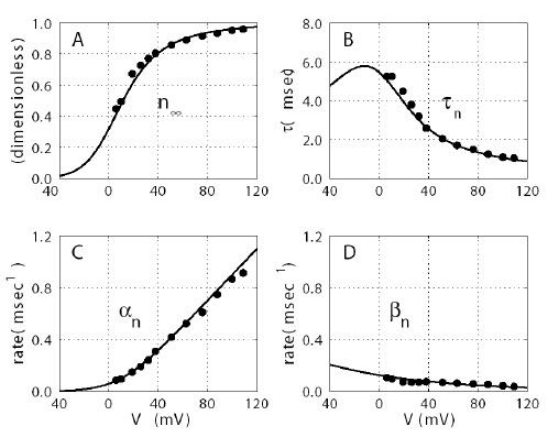
\includegraphics[scale=0.5]{../Figuras/medidasExperimentales.png}
 \caption{Medición experimental de los parámetros y ajuste manual de curvas. Imagen de Nelson 2004}
 \label{fig:voltajeAB}
\end{figure}

Con estas medidas experimentales ellos dan con curvas paramétricas ajustadas a los factores \(\alpha\) y \(\beta\) expresadas de la siguiente forma:

\begin{align*}
\alpha_{n}&=\dfrac{0.01(10-V)}{e^{\left(\dfrac{10-V}{10}\right)}-1}           &  \beta_{n}&=0.125e^{-\dfrac{V}{80}}\\
\alpha_{m}&=\dfrac{0.01(25-V)}{e^{\left(\dfrac{25-V}{10}\right)}-1}                    &  \beta_{m}&=4e^{-\dfrac{V}{18}}\\
\alpha_{h}&=0.07 e^{-\left(\dfrac{V}{20}\right)}              &  \beta_{h}&=\dfrac{1}{e^{\left(\dfrac{30-V}{10}\right)}+1}
\label{eq:curvas}
\end{align*}


Ahora veamos las gráficas de la dinámica del disparo pero ya con los las compuertas del potasio y sodio interactuando al mismo tiempo, en las figuras \ref{fig:voltajeActInac} y \ref{fig:voltajeActInac1}


\begin{figure}[h]
 \centering
 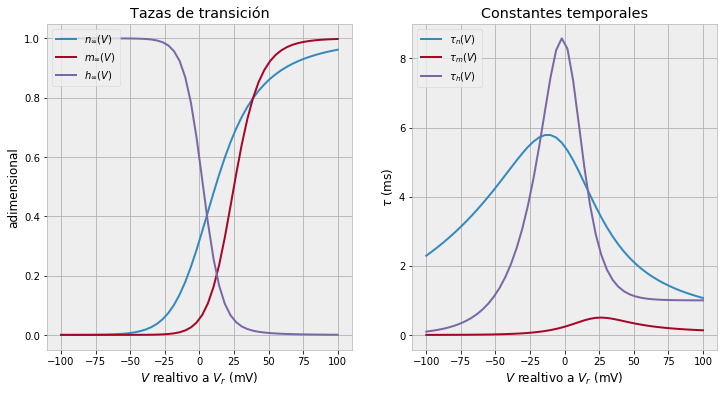
\includegraphics[scale=0.6]{../Figuras/actinac.png}
 \caption{Activación e inactivación de los canales. Del lado izquierdo vemos que alrededor de los -50 mV aumenta la probabilidad que las compuertas de potasio abran y los potasios salgan, el sodio tarda un poco más en reaccionar para dejar entrar a los sodios, y la probabilidad que quede no bloqueado disminuye, hasta bloquear por completo a los iones de sodio alrededor de los 50 mV. Del lado derecho vemos como \(\tau\), va interactuando conforme al voltaje, el Na+ reacciona rápidamente ante él impuso pues regresa rápidamente a su estado de equilibrio, esto indica porque aún que el sodio abre sus compuertas, la compuerta de bloqueo se cierra rápidamente, dejando inactivado el canal, luego el K+ reacciona más lentamente para regresar a su estado de equilibrio dejando más tiempo activado el canal y salgan los potasios.}
 \label{fig:voltajeActInac}
\end{figure}


\begin{figure}[H]
 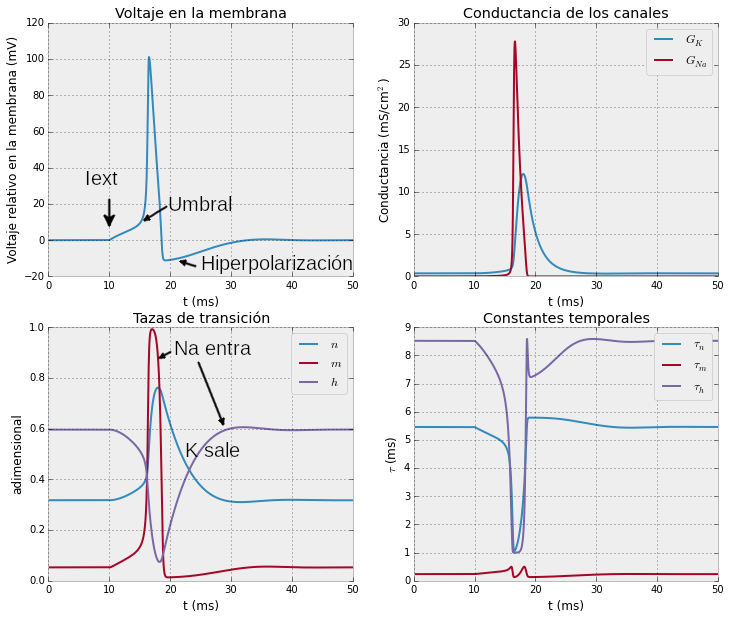
\includegraphics[scale=0.6]{../Figuras/disparo.png}
 \caption{Medidas experimentales del estímulo y la reacción de todos los componentes de la membrana. El origen en estás gráficas realmente esta representando el punto de equilibrio que es alrededor de los -70mV. Del lado superior izquierdo mostrando como cambia el voltaje de la membrana respecto al tiempo, del lado superior derecho el comportamiento de la conductancia de los canales mostrando que aunque la conductancia del sodio reacciona más, es más breve, mientras que el potasio reacciona en menor medida pero durante más tiempo. En la parte inferior derecha la taza de transición de las compuertas n,m y h, mostrando que en cuando llega el impulso el primero en reaccionar es el sodio permitiendo que entre muy brevemente el sodio e inactivandose casi inmediatemente después, mientras que en ese momento los potasios se están liberando hacia la parte exterior de la meurona. Finalmente del lado inferior izquierdo mostrando como se comporta las constantes temporales, mostrando que las compuertas de activación de sodio no son tan afectadas comparado a la compuerta de bloqueo, notando algunos cambio bruscos en esta, mientras que el potasio si se nota más afectado y durante más tiempo pero recuperandose sin cambios bruscos. }
 \label{fig:voltajeActInac1}
\end{figure}




\section{Simulación usando el método de Euler}

En esta sección se listará como estamos resolviendo las ecuaciones diferenciales, para tener una simulación numérica y se trata del algoritmo de integración \footnote{Hodgkin-Huxley Simulation Using Euler's Method lo puedes encontrar en la siguiente liga \url{https://webpages.uidaho.edu/rwells/techdocs/Biological\%20Signal\%20Processing/Chapter\%2003\%20The\%20Hodgkin-Huxley\%20Model.pdf}}. Las gráficas de la sección anterior se obtuvieron con el método de Euler que se describe más adelante.

\begin{algorithm}
  \caption{Algoritmo de integración de Euler [Wells pp51].}\label{AIE}
  \begin{algorithmic}[1]
    \Function{INTEGRADISPARO}{$T,\Delta T,V_{0},I_{ext}(t)$}
    \State Inicializar arreglos de logitud T: $T[],V[],n[],m[],h[],G_{Na}[],G_{K}[],\tau_{n}[],\tau_{m}[],\tau_{h}[] \gets arreglo[numeroDePasos] $
    \State  $V[0] \gets V_{0}$
    \For {$ t = 0  a  t = T cada \Delta t $}
        \State Calcular $\alpha_{n}, \beta_{n}, \alpha_{m}, \beta_{m},\alpha_{h}, \beta_{h} $ utilizando $V(t)$.
        \State Calcular las tres $\tau_{x} $ y $x^\infty $ apartir de las anteriores.
        \State Calcular las probabilidades de las compuertas $n, m, h, $ utilizando las ecuaciones en diferencias en su forma matricial $\Pi(t + \Delta t) = A_{\pi}\Pi(t) + B_{\pi}$.
        \State Calcular $G_{Na} = g_{Na}m^3h $ y $G_{K} = g_{K}n^4 $.
        \State Almacenar los resultados de este paso en los arreglos $T[], V[], n[], m[], h[], G_{Na}[], G_{K}[], \tau_{n}[], \tau_{m}[], \tau_{h}[] $
        \State $I_{ext} \gets I_{ext}(t) $
        \State Calcular $V_{m} (t + \Delta t) $
    \EndFor
    \State Devolver los arreglos $T[],V[],n[],m[],h[],G_{Na}[],G_{K}[],\tau_{n}[],\tau_{m}[],\tau_{h}[] $ con los resultados para los tiempos $[0,T] $
    \EndFunction
  \end{algorithmic}
\end{algorithm}


Comenzamos con un valor inicial y a partir de ahí empleamos las ecuaciones, para calcular las tangentes, aproximamos a la curva con su tangente.

Para la función \textproc{INTEGRADISPARO} necesitamos cuatro valores de entrada que van a provocar diferentes comportamientos:

\begin{enumerate}
 \item $T$ nos indica durante cuánto tiempo queremos correr la simulación.
 \item $\Delta T $ nos indica que tan finos queremos que sean los pasos recordemos que vamos a aproximar la función con segmentos de recta siguiendo la tangente. Si hacemos pasos demasiado pequeños nos vamos a tardar demasiado en hacer el cómputo.
 \item $V_{0} $ es el voltaje inicial en donde empieza nuestra simulación donde estaba en nuestra neurona cuando empezamos a trabajar.
 \item $I_{ext}(t) $ es la corriente externa, de qué magnitud fue el toque que le estamos dando en este momento al axón 

\end{enumerate}

A partir de los elementos iniciales proporcionados ya podemos calcular lo demás. Vamos a querer guardar lo que está ocurriendo para todos los tiempos desde cero hasta t en cada delta, y lo vamos a hacer en forma de arreglos donde en la posición [0], está la primera medición en t=0 y la posición t está la medición en el tiempo t. Vamos a tener toda una serie de puntos donde estamos guardando estos pasos para inicializarlo. 

Sabemos que necesitamos es un primer valor a partir del cual vamos a calcular la tangente y vamos a ir aproximando lo demás, entonces para eso queríamos \emph{el voltaje inicial}, como nosotros sabemos donde estaba en reposo nuestra célula originalmente, vamos a poder guardar ese voltaje como el primer valor para nuestra simulación. Ahora todos los demás elementos como $\alpha$s y $\beta$s y etc. se pueden calcular si ya conocíamos ese voltaje inicial, entonces a partir de este momento podemos repetir el mismo ciclo tantas veces como sea necesario para cubrir, el intervalo. 
Desde el tiempo inicial hasta el tiempo t, brincando de delta T en delta T. 
Entonces dado un voltaje vamos a calcular las diferentes \(\alpha\)s que son las que se medían experimentalmente originalmente utilizando las ecuaciones  de las curvas paramétricas ajustadas \ref{eq:curvas} (paso 5).

Ya calculadas las alfas y betas ahora si se puede calcular las $\tau$ , $n^{\infty}$, $m^{\infty}$, $h^{\infty}$ (paso 6).
Teniendo estas entonces podemos calcular las probabilidades para las compuertas n, m, h usando las ecuaciones en diferencias en forma matricial, estas matrices se pueden expresar como \ref{fig:matriX}.

\begin{figure}[H]
 \centering
 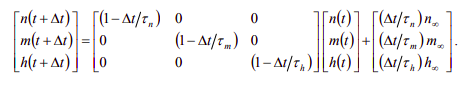
\includegraphics[scale=0.7]{../Figuras/matrix.png}
 \caption{Forma matricial para el cálculo de las probabilidades de las compuertas n, m, h.}
 \label{fig:matriX}
\end{figure}

Ahora esta parte fue importante sobre todo por el asunto de las pérdidas numéricas, recordemos que la computadora tiene una representación en punto flotante, lo cual quiere decir que un número real no se puede representar en la computadora, esto es importante por el problema del truncamiento, cada vez que se truncan dígitos al momento de calcular estamos perdiendo precisión, por esto es importante la forma en la que se procede a hacer los cálculos porque puede que se llegue a resultados un tanto distintos a los deseados aunque los cálculos sean correctos. 

Ya teniendo estos datos podemos fácilmente calcular las conductancias, simplemente sustituyendo los valores (paso 8).

Es bueno una vez que ya terminamos de calcular estos términos que se van a necesitar en la ecuación principal  \ref{eq:corrientesEnLaMembrana2} que es la del voltaje de la membrana,  ir almacenando en los \emph{resultados temporales} dentro de nuestros arreglos en la casilla que les corresponda, para ese momento (paso 8). En el paso 9, es donde ya vamos a utilizar \emph{la corriente externa} para meterla en la ecuación diferencial para el voltaje. Una vez que tengamos esto tenemos que repetirlo para cada paso, se está calculando el tiempo t,  entonces conforme avance el tiempo, va a dar el siguiente valor del voltaje, ya teniendo el siguiente valor del voltaje se va a poder usar para el siguiente paso ("como valor inicial nuevo") y así nos vamos a seguir todo el tiempo. 
Terminando el tiempo asignado a la simulación, tenemos ya los arreglos llenos de los datos que nos van a poder permitir graficar, qué fue lo que sucedió en cada tiempo, con cada canal y es precisamente  así que se puede graficar las mediciones presentadas en la sección anterior.


\section{Información condificada en las dendritas}

En esta última sección de este capítulo, se va a tratar el cómputo en las neuronas, que vamos a simplificar para poder modelar las neuronas artificiales. Ya vimos detalladamente que pasa a lo largo del axón de la neurona, se ha mencionado que son quienes conforman la región que recibe la información (disparos / pulsos). Estos mandados desde los botones de las terminales de las neuronas presinápticas y son las dendritas las encargadas de enviar estas señales hasta el soma de la neurona y hacer que estas señales químicas se transformen o no en impulsos eléctricos. Ahora la siguiente cuestión es ¿Podemos hacer que se dispare más de una vez (con el mismo estímulo)?.

Los disparos que produzca una neurona depende fuertemente de la interacción con sus neuronas vecinas. Recordemos que durante el período refractario lo que sucede, es que cuando se acumula información en las periferias del cuerpo de la neurona a través de las dendritas y de su cuerpo es porque; está recibiendo información de neuronas vecinas y eso va a hacer que dispare.

Algunas neuronas tienen el periodo de refractario muy pequeño y disparan frecuentemente, por las conexiones que tienen con sus vecinas, son neuronas que mandan frecuentemente información y a veces pueden lanzar una serie de pulsos muy seguidos, en
otras ocasiones puede haber interrupciones entre estas series de pulsos (ver imagen \ref{fig:neuronStaining}, en caso de los seres humanos podemos referirnos a las neuronas motoras que están en constante recepción y transmisión de información).

\begin{figure}[h]
 \centering
 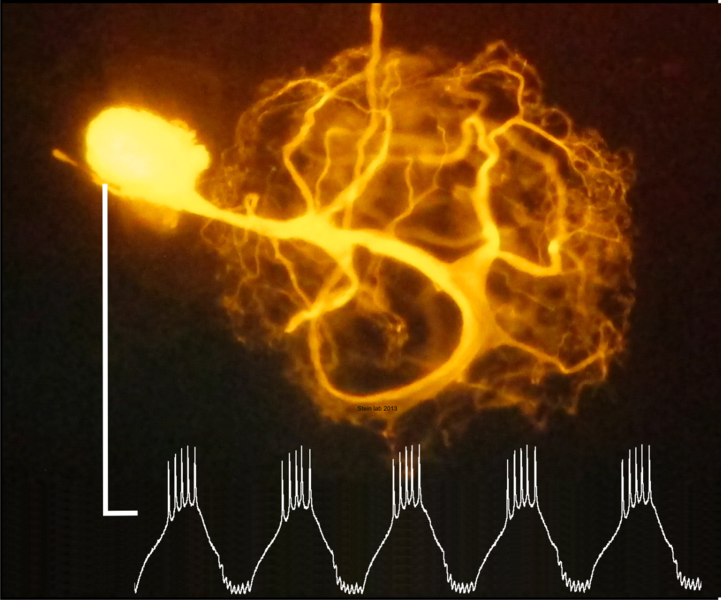
\includegraphics[scale=0.7]{../Figuras/neuron_staining_and_recording.png}
 \caption{Disparos de una neurona, Wstein, 14 September 2013, Wikimedia Commons. Esta foto muestra la neurona de cangrejo que se tiñó mediante la inyección intracelular de un colorante fluorescente. El recuadro muestra una grabación de las oscilaciones rítmicas del potencial de membrana. Las grabaciones fueron realizadas por Christopher Goldsmith en el laboratorio de Wolfgang Stein en la Universidad Estatal de Illinois, \url{https://upload.wikimedia.org/wikipedia/commons/c/ca/PD_neuron_staining_and_recording.png} , CC BY-SA 3.0.}
 \label{fig:neuronStaining}
\end{figure}

Por otro lado, hay otras neuronas que son muchísimo más pasivas y disparan muy rara vez (neuronas que están a niveles más altos, como reconocimiento de olores, colores, imágenes). Y también nos encontramos con casos donde aparentemente una neurona no reacciona ante ningún estímulo, hasta que pasa un estímulo muy especifico \footnote{Neuronas individuales que forman conceptos abstractos, responden por ejemplo, al nombre de un ser humano. Es así como se descubrió la neurona ‘Jennifer Aniston’, que disparaba cada vez que el retrato de la actriz se mostraba a los sujetos. Estas neuronas, que responden ante la presentación de algunas imágenes recibieron la denominación de“células abuelas”.} y está dispara (neuronas conceptuales o aisladas). La comunidad científica aún no se atreve a afirmar si este tipo de neurona solo dispara ante ese estímulo específico, o simplemente se trata de un evento que cumple con todas las condiciones para que esta neurona reaccione y mande un pulso. Cabe mencionar que estas neuronas se encuentran en las capas más altas de abstracción de procesamiento del cerebro \footnote{En la siguiente liga se puede encontrar información más detallada acerca de la investigación con estas neuronas: \url{https://www.nature.com/articles/s41598-020-64466-7}}. Este tipo de diferencias entre neuronas te será más fácil recordar si regresas a la última sección del primer capítulo donde se encuentra un diagrama de los procesos de información en los que puede invertir una neurona, este diagrama es \ref{fig:zonasFun}.

En este momento notamos la gran importancia de la codificación de la información en las redes neuronales de un cerebro. Donde la frecuencia de potenciales de acción nos muestran, ciertos patrones que nos indican el nivel de abstracción al que está respondiendo la neurona y el tipo de información que ayuda codificar o decodificar. 

Teniendo ahora noción del papel que juegan los patrones de la frecuencia de disparos, se han hecho numerosas investigaciones acerca de estos. En un intento de entender mejor como es que un cerebro recibe la información desde el exterior, procesa y finalmente provoca ciertas reacciones ante el estímulo. En la siguiente imagen \ref{fig:simpleModel} que es el resultado de un artículo donde se utilizaron diferentes métodos para simular disparos de neuronas y notamos la clasificación de estos patrones que se dan ante ciertos estímulos. Cada uno de estos patrones, están codificando cosas distintas, donde una misma neurona podría alternar entre diferentes patrones dependiendo de cuál es el estímulo que está recibiendo.
Si bien ha habido algunas propuestas donde se tratan de hacer neuronas artificiales que tomen en cuenta la frecuencia de disparos aún hay un amplio campo de investigación en este tema.

\begin{figure}[h]
 \centering
 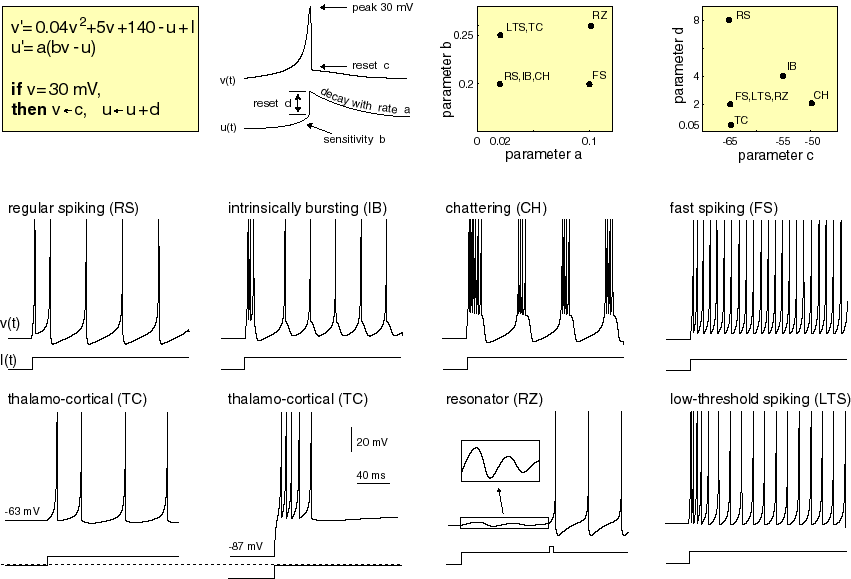
\includegraphics[scale=0.5]{../Figuras/Simple_Model_of_Spiking_Neurons.png}
 \caption{Diferentes patrones de disparo (simulados), Eugene M. Izhikevich, 2003, The Neurosciences Institute, \url{http://www.izhikevich.org/publications/spikes.html}}
 \label{fig:simpleModel}
\end{figure}

Por último mostremos la situación del sistema auditivo con la siguiente imagen \ref{fig:sonidoDisp}:

\begin{figure}[H]
 \centering
 \includegraphics[scale=0.4]{../Figuras/Localización_del_sonido_por_disparidad.png}
 \caption{Localización del sonido por disparidad, Ian Stevenson, 7 enero 2008, El sistema auditivo registra y analiza pequeñas diferencias en el tiempo de llegada de los sonidos a los dos oídos para estimar la dirección desde la cual el sonido es emitido, \url{http://www.scholarpedia.org/w/images/4/4d/JeffressFig1.png}}
 \label{fig:sonidoDisp}
\end{figure}

La imagen muestra cómo computan las neuronas, este ejemplo se trata del sistema de audio humano. Cuando nosotros oímos podemos tratar de inferir aproximadamente desde donde está siendo emitido el sonido y eso se logra gracias a que tenemos neuronas conectadas al área auditiva (tanto con el oído derecho como con el oído izquierdo). La señal auditiva va a tardar más en llegar a un oído que al otro, dependiendo de su posición en el espacio, por lo que el cerebro siempre tratar de calcular ese desfase.  
En el esquema se representa como dentro del espacio de una persona se encuentra una fuente de sonido. Dependiendo de la dirección que provenga (izquierda o derecha), las neuronas receptoras de cada oído harán un cálculo rápido de la distancia a la que se percibió la señal, estás llegaran al cerebro y en algún punto enlazaran con neuronas donde estás cuentan las diferencias de distancias percibidas hasta llegar a dar con el resultado, dándonos a saber cuáles receptores (izquierda o derecha) están más cerca de la señal, y así ubiquemos desde donde proviene el sonido.


